\clearpage
\section{Data analysis Pernis Refinery}\label{Pernis}
In this section, a descriptive analysis of EF measurements from a fuel gas in the Pernis refinery is presented. 
From 2014 to 2020, the fuel gas stream has been sampled at more or less regular intervals albeit with certain longer periods without any measurements. For each sample, the EF is measured based on a full analysis of the composition of the fuel gas in the laboratory. There is considerable variability in the EF over time (figure~\ref{fig:timeseries}), which is believed to be a reflection of the variability in process conditions, as the measurement uncertainty is small. The annual variability in EF, due to temporal variability in the composition of the fuel gas, is given in figure~\ref{fig:Pernis_hist}.

\begin{figure}[h]
	\centering
	\includegraphics[width=0.65\textwidth]{graphs/timeseries.pdf}
	\caption{Time series plot of EF, measured on samples taken from the flow of a fuel gas at the Pernis refinery.}
	\label{fig:timeseries}
\end{figure}

\begin{figure}[h]
	\centering
	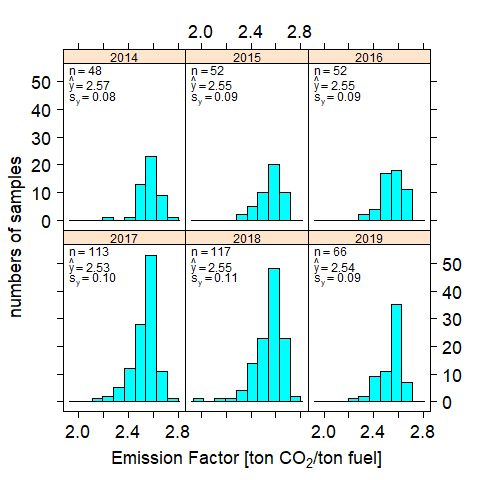
\includegraphics[width=0.65\textwidth]{graphs/Pernis_hist.pdf}
	\caption{Frequency histograms of EF, measured on samples taken from the flow of a fuel gas at the Pernis refinery. Indicated are the annual number of samples $n$, the annual standard deviation in measured EF ($\sigma_y$) and the annual average EF ($\hat{y}$).}
	\label{fig:Pernis_hist}
\end{figure}

The EF correlates very strongly with the Stoichiometric Air Requirement (SAR; figure~\ref{fig:SAR_y_peryear}) and less strongly with Lower Heating Value (LHV; figure~\ref{fig:LHV_y_peryear}). Estimates of SAR and LHV are based on the composition of the sample of fuel gas as determined in the laboratory. As such, these variables are therefore not directly useful as auxiliary variables. However, these relationships may provide clues to potential candidates for high-frequency online measurements that may correlate well with EF. SAR may be directly estimated based on a mass spectrometry device (see e.g. \cite{Merriman}), and it is worth investigating if oxygen analyzers or calorimeters correlate well with either SAR or LHV.

\begin{figure}[h]
	\centering
	\includegraphics[width=0.65\textwidth]{graphs/SAR_y_peryear.pdf}
	\caption{Scatterplot of EF against Stoichiometric Air Requirement (SAR), with Pearson correlation coefficients ($\rho$). }
	\label{fig:SAR_y_peryear}
\end{figure}


\begin{figure}[h]
	\centering
	\includegraphics[width=0.65\textwidth]{graphs/LHV_y_peryear.pdf}
	\caption{Scatterplot of EF against Lower Heating Value (LHV), with Pearson correlation coefficients ($\rho$). }
	\label{fig:LHV_y_peryear}
\end{figure}

%\begin{figure}[h]
%	\centering
%	\includegraphics[width=0.7\textwidth]{graphs/SAR_y_residuals.pdf}
%	\caption{ }
%	\label{fig:SAR_y_residuals}
%\end{figure}
The residuals of a linear model of EF on SAR correlate strongly with molar weight as measured by an analyser which is already online in the fuel gas stream at the Pernis refinery (figure~\ref{fig:SAR_y_residuals_molweight_peryear}). A multiple linear regression model of EF on SAR and molar weight yields predictions that correlate very strongly with measured EF (figure~\ref{fig:SAR_y_predicted_SAR_molweight_peryear}). This is encouraging because, if a device can be found which can measure online a variable which correlates with SAR or LHV, then this may result in a model with good predictive performance in combination with online molar weight measurements.

\begin{figure}[h]
	\centering
	\includegraphics[width=0.65\textwidth]{graphs/SAR_y_residuals_molweight_peryear.pdf}
	\caption{ Scatterplot of the residuals of a linear regression model of EF on SAR, versus molar weight. }
	\label{fig:SAR_y_residuals_molweight_peryear}
\end{figure}

\begin{figure}[h]
	\centering
	\includegraphics[width=0.65\textwidth]{graphs/SAR_y_predicted_SAR_molweight_peryear.pdf}
	\caption{Scatterplot of measured versus predicted EF. The EF was predicted using a linear regression model with SAR and molar weight as covariates. Indicated on the graphs are Pearson correlation coefficients ($\rho$). }
	\label{fig:SAR_y_predicted_SAR_molweight_peryear}
\end{figure}

A time series plot of the residuals of the multiple linear regression model of EF on SAR and molar weight indicates that there are still some unexplained trends in the EF measurements (figure~\ref{fig:SAR_residuals_SAR_molweight_timeseries}). For example, there is a consistent deviation between predicted and measured EF in 2019. This, however, does not have to lead to a deterioration of the uncertainty of the estimate of the annual average, as long as the annual average EF is based on a combination of direct EF measurements in the laboratory and the auxiliary variable(s).

\begin{figure}[h]
	\centering
	\includegraphics[width=0.65\textwidth]{graphs/SAR_residuals_SAR_molweight_timeseries.pdf}
	\caption{Time series plot of the residuals of a multiple linear regression model of EF on SAR and molar weight. }
	\label{fig:SAR_residuals_SAR_molweight_timeseries}
\end{figure}

An exploratory data analysis (not shown in this report) indicated that the residuals of the multiple linear regression model of EF on SAR and molar weight correlate with ethylene and propylene concentrations in the fuel gas. Based on these two additional variables, the predictive model for EF could be further improved. However, this is not further discussed or illustrated here.
%
%\begin{figure}[h]
%	\centering
%	\includegraphics[width=0.65\textwidth]{graphs/SAR_y_predicted_SAR_molweight_Pr_Eth_peryear.pdf}
%	\caption{ }
%	\label{fig:SAR_y_predicted_SAR_molweight_Pr_Eth_peryear}
%\end{figure}
%
%\begin{figure}[h]
%	\centering
%	\includegraphics[width=0.65\textwidth]{graphs/Residuals_SAR_molweight_Pr_Eth_timeseries.pdf}
%	\caption{ }
%	\label{fig:Residuals_SAR_molweight_Pr_Eth_timeseries}
%\end{figure}
